% \iffalse
\let\negmedspace\undefined
\let\negthickspace\undefined
\documentclass[journal,12pt,twocolumn]{IEEEtran}
\usepackage{cite}
\usepackage{amsmath,amssymb,amsfonts,amsthm}
\usepackage{algorithmic}
\usepackage{graphicx}
\usepackage{textcomp}
\usepackage{xcolor}
\usepackage[justification=centering]{caption}
\usepackage{txfonts}
\usepackage{listings}
\usepackage{enumitem}
\usepackage{mathtools}
\usepackage{gensymb}
\usepackage{comment}
\usepackage[breaklinks=true]{hyperref}
\usepackage{tkz-euclide} 
\usepackage{listings}
\usepackage{gvv}                                        
\def\inputGnumericTable{}                                 
\usepackage[latin1]{inputenc}                                
\usepackage{color}                                            
\usepackage{array}                                            
\usepackage{longtable}                                       
\usepackage{calc}                                             
\usepackage{multirow}                                         
\usepackage{hhline}                                           
\usepackage{ifthen}                                           
\usepackage{lscape}

\newtheorem{theorem}{Theorem}[section]
\newtheorem{problem}{Problem}
\newtheorem{proposition}{Proposition}[section]
\newtheorem{lemma}{Lemma}[section]
\newtheorem{corollary}[theorem]{Corollary}
\newtheorem{example}{Example}[section]
\newtheorem{definition}[problem]{Definition}
\newcommand{\BEQA}{\begin{eqnarray}}
\newcommand{\EEQA}{\end{eqnarray}}
\newcommand{\define}{\stackrel{\triangle}{=}}
\theoremstyle{remark}
\newtheorem{rem}{Remark}
\begin{document}

\bibliographystyle{IEEEtran}
\vspace{3cm}

\title{11.9.5.31}
\author{MANOJ KUMAR (EE23BTECH11211)}
\maketitle
\newpage

\bigskip

\renewcommand{\thefigure}{\theenumi}
\renewcommand{\thetable}{\theenumi}
\textbf{Question 31:}
A manufacturer reckons that the value of a machine, which costs him Rs.$15625$, will depreciate each year by $20\%$.Find the estimated value at the end of 5 years.\\
\solution\\
\begin{table}[!ht]
\renewcommand\thetable{1}
   \centering
\begin{tabular}{|c|c|c|}
    \hline
      \text{Symbol} & \text{Value} & \text{Description} \\
    \hline
        $x(0)$ & $-6$ & first term of AP\\
   \hline
        $d$ & $\frac{1}{2}$ & common difference of AP\\
   \hline
         $n+1$ & $?$ & number of terms \\
    \hline 
    $x(n)$ & $x(0)+nd$ & nth term of the AP \\
    \hline 

  \end{tabular}\\
  \caption{Input data}
  \label{Input data}
\end{table}

 \begin{align}
     x(n) &= 15625 \Big(1-\frac{1}{5}\Big)^{n}u(n)
 \end{align}
 Result:
 \begin{align}
  a^nu(n)\system{Z} \frac{1}{\brak{1-az^{-1}}}\quad\abs{z}>{a} 
  \label{eq:11.9.5.31.2}	 
  \end{align}
 From \eqref{eq:11.9.5.31.2}
\begin{align}
    X(Z) &= \frac{15625}{1 - \Big(1-\frac{1}{5}\Big)z^{-1}} \quad\abs{z}>\frac{4}{5}
\end{align}
 \begin{figure}[!ht]
    \centering
    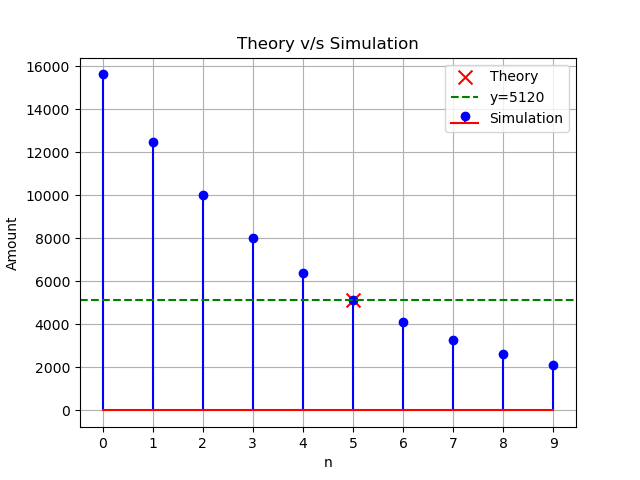
\includegraphics[width=1\linewidth]{figs/plot2.png}
    \caption{Theory matches with simulated values}
    \label{fig:enter-label}
\end{figure}
\end{document}
